\documentclass[
12pt, % tamanho da fonte
openright, % capítulos começam em página ímpar (insere página vazia caso preciso)
oneside, % oposto a twoside (imprime somente em um lado da folha)
a4paper, % tamanho do papel
chapter=TITLE, % títulos de capítulos convertidos em letras maiúsculas
section=TITLE, % títulos de seções convertidos em letras maiúsculas
english, % idioma adicional para hifenização
french, % idioma adicional para hifenização
spanish, % idioma adicional para hifenização
brazil % último idioma é o principal do documento
]{abntex2-uepg}

\usepackage{lmodern} % usa a fonte Latin Modern			
\usepackage[T1]{fontenc} % seleção de códigos fonte
\usepackage[utf8]{inputenc} % codificação do documento (conversão automática dos acentos)
\usepackage{indentfirst} % indenta o primeiro parágrafo de cada seção.
\usepackage{color} % controle das cores
\usepackage{graphicx} % inclusão de gráficos
\usepackage{uepg}
\usepackage{lipsum}		
\usepackage{amssymb}
\usepackage{amsmath}
\usepackage{setspace}
\usepackage{lscape}
\usepackage{longtable}	
\usepackage{listings}

\AtBeginDocument{%
  \counterwithout{lstlisting}{chapter}% remove chapter binding
  \renewcommand{\thelstlisting}{\arabic{lstlisting}}% show 1,2,3...
  \setcounter{lstlisting}{0}% first one becomes 1
}

\usepackage{gantt}
\usepackage{xcolor}
\usepackage[bottom=2cm,top=3cm,left=3cm,right=2cm]{geometry}
\usepackage{titlesec}
\usepackage{caption}
\usepackage[brazilian,hyperpageref]{backref} % paginas com as citações na bibl
\usepackage[
alf,
abnt-emphasize = bf, % destaca o titulo da revista ou livro em negrito
abnt-etal-list = 3, % trabalhos com mais de 3 autores recebem et al.
abnt-etal-text = it, % escreve o et al., em italico
abnt-and-type = &, % usa o carater '&' no lugar de 'e' para mais de um autor
abnt-last-names = abnt, % trata sobrenomes 'estritamente' conforme a ABNT
abnt-repeated-author-omit = no
]{abntex2cite}

\usepackage{float}

% mantém o texto justificado
\usepackage[none]{hyphenat}
\tolerance=1000
\emergencystretch=3em

\captionsetup[table]{
	singlelinecheck=false, % alinha o caption da tabela à esquerda
}
\captionsetup[figure]{
	singlelinecheck=false, % alinha o caption da figura à esquerda
}

\titlespacing*{\subsection}{0pt}{2.5ex plus 1ex minus .2ex}{2.5ex plus .2ex} 

\setlength\afterchapskip{\lineskip}

\definecolor{codegray}{rgb}{0.5,0.5,0.5}

\newcommand{\fontealgoritmo}[1]{%
    \begingroup
    \captionsetup{
        justification=raggedright,
        singlelinecheck=false,
        skip=0pt
    }
    \setlength{\abovecaptionskip}{-5pt}
    \fonte{#1}
    \addvspace{1.0\baselineskip}
    \endgroup
}

\captionsetup[lstlisting]{
    justification=raggedright,
    singlelinecheck=false
}

\lstdefinestyle{mystyle}{
    basicstyle=\fontfamily{phv}\selectfont\footnotesize,
    commentstyle=\color{codegray},
    keywordstyle=\bfseries,
    stringstyle=\normalfont,
    numbers=none,
    breakatwhitespace=false,
    breaklines=true,
    keepspaces=false,
    showspaces=false,
    showstringspaces=false,
    showtabs=false,
    tabsize=4,
    frame=tb,
    captionpos=t
}

\lstset{style=mystyle}

\lstset{
    inputencoding=utf8,
    extendedchars=true,
    literate=
        {á}{{\'a}}1
        {é}{{\'e}}1
        {í}{{\'i}}1
        {ó}{{\'o}}1
        {ú}{{\'u}}1
        {ã}{{\~a}}1
        {õ}{{\~o}}1
        {â}{{\^a}}1
        {ê}{{\^e}}1
        {ô}{{\^o}}1
        {ç}{{\c{c}}}1
}

\lstdefinelanguage{Rust}{
    keywords={
        as, break, const, continue, crate, else, enum, extern, false,
        fn, for, if, impl, in, let, loop, match, mod, move, mut, pub,
        ref, return, self, Self, static, struct, super, trait, true,
        type, unsafe, use, where, while, async, await, dyn
    },
    sensitive=true,
    comment=[l]{//},
    morecomment=[s]{/*}{*/},
    morestring=[b]",
}

\lstdefinelanguage{JavaScript}{
    keywords={
        var, let, const, function, return, if, else, for, while, do,
        break, continue, switch, case, default, new, delete, typeof,
        instanceof, in, of, this, class, extends, super, import, export,
        from, async, await, true, false, null, undefined, try, catch,
        finally, throw
    },
    sensitive=true,
    comment=[l]{//},
    morecomment=[s]{/*}{*/},
    morestring=[b]",
    morestring=[b]',
}

\renewcommand{\backrefpagesname}{Citado na(s) página(s):~} % configurações do pacote backref, usado sem a opção hyperpageref de backref
\renewcommand{\backref}{} % texto padrão antes do número das páginas
\renewcommand*{\backrefalt}[4]{ % define os textos da citação
	\ifcase #1 %
	Nenhuma citação no texto.
	\or
	Citado na página #2.
	\else
	Citado #1 vezes nas páginas #2.
	\fi
}

\renewcommand{\rmdefault}{phv} % arial
\renewcommand{\sfdefault}{phv} % arial

\renewcommand{\lstlistingname}{Algoritmo} % formatação de código fonte
\renewcommand{\lstlistlistingname}{Lista de algoritmos}

\autor{Carlos Eduardo Varela de Almeida\\Mateus Enrick Pitura\\Raissa Mayara Moreira}
\data{2026}
\local{Ponta Grossa}
\orientador{Prof. Dr. Luciano José Senger}
\preambulo{Trabalho de conclusão de Curso apresentado ao Curso de Engenharia de Software da Universidade Estadual de Ponta Grossa, como requisito parcial para obtenção do título de Bacharel em Engenharia de Software.}
\titulo{Impacto do WebAssembly no desempenho de aplicações Rust}
\tipotrabalho{Trabalho de Conclusão de Curso}

\definecolor{blue}{RGB}{41,5,195}

\makeatletter
\hypersetup{
	pdftitle={\@title}, 
	pdfauthor={\@author},
	pdfsubject={\imprimirpreambulo},
	pdfcreator={LaTeX with abnTeX2},
	pdfkeywords={abnt}{latex}{abntex}{abntex2}{trabalho acadêmico}, 
	colorlinks=true,       		
	linkcolor=black,
	citecolor=black,
	filecolor=magenta,
	urlcolor=black,
	bookmarksdepth=4
}
\makeatother

% posiciona figuras e tabelas no topo da página quando adicionadas sozinhas, em um página em branco. Ver https://github.com/abntex/abntex2/issues/170
\makeatletter
	\setlength{\@fptop}{5pt}
\makeatother

% possibilita criação de Quadros e Lista de quadros. Ver https://github.com/abntex/abntex2/issues/176
% \newcommand{\quadroname}{Quadro}
% \newcommand{\listofquadrosname}{Lista de quadros}

% \newfloat[chapter]{quadro}{loq}{\quadroname}
% \newlistof{listofquadros}{loq}{\listofquadrosname}
% \newlistentry{quadro}{loq}{0}

% configurações para atender às regras da ABNT
% \setfloatadjustment{quadro}{\centering}
% \counterwithout{quadro}{chapter}
% \renewcommand{\cftquadroname}{\quadroname\space} 
% \renewcommand*{\cftquadroaftersnum}{\hfill--\hfill}

\setfloatlocations{quadro}{hbtp} % ver https://github.com/abntex/abntex2/issues/176

% tamanho do parágrafo
\setlength{\parindent}{1.3cm}

% controle do espaçamento entre um parágrafo e outro
\setlength{\parskip}{0.2cm}

% espaçamento simples entre parágrafos
\setlength{\parskip}{0cm}
% espaçamento entre o título e o primeiro parágrafo do texto
\setlength\afterchapskip{18pt}

\makeindex % compila o índice

% lista de códigos
\newlistof{lstlistoflistings}{lol}{\lstlistlistingname}

\begin{document}
	\selectlanguage{brazil}
	\frenchspacing 
	
	\imprimircapa
	
	% (o * indica que haverá a ficha bibliográfica)
	\imprimirfolhaderosto

	% \input{content/dedicatoria}
	
	\begin{agradecimentos}
	Expressamos nossos sinceros agradecimentos ao Prof. Dr. Luciano José Senger pela orientação dedicada ao longo deste trabalho, conduzida com atenção, paciência e compromisso acadêmico. Suas contribuições foram essenciais para o desenvolvimento e a conclusão desta pesquisa.

Aos nossos pais e amigos, manifestamos nossa profunda gratidão pelo apoio incondicional, incentivo constante e confiança depositada durante toda a trajetória acadêmica. A presença de vocês foi fundamental para a concretização deste trabalho.
	\end{agradecimentos}
	
	% \input{content/epigrafe}

	\setlength{\absparsep}{18pt}
	\begin{resumo}
	O WebAssembly tem se consolidado como uma alternativa para execução de aplicações de alto desempenho em navegadores \emph{web}, permitindo a utilização de linguagens compiladas além da linguagem JavaScript. Entre elas, o Rust destaca-se pela eficiência computacional e sua segurança de memória, tornando-se uma opção importante para o desenvolvimento de aplicações executadas no ambiente \emph{web}. Neste contexto, este trabalho realiza uma análise comparativa entre a execução nativa de algoritmos implementados em Rust e a execução dos mesmos algoritmos compilados para WebAssembly. Para a realização dos experimentos, foram selecionados algoritmos representativos de diferentes classes de problemas computacionais a partir do The Computer Language Benchmarks Game. As implementações foram adaptadas para os dois ambientes de execução e avaliadas em ambiente controlado por contêineres Docker, com análise de tempo de execução e consumo de memória. Os resultados mostram que o Rust nativo foi mais rápido em todos os algoritmos avaliados, com \emph{overhead} do WebAssembly variando de 10,9\% a 126,9\% conforme o algoritmo, com mediana de 21,2\%. Em relação à memória, o ambiente WebAssembly manteve cerca de 210 MiB em repouso, devido ao navegador e à ferramenta de automação, o que tornou necessário o uso das métricas de \emph{baseline} e consumo líquido para isolar o consumo dos algoritmos, que foi reduzido na maioria dos casos e maior no mandelbrot, nos dois ambientes, em valor compatível com o \emph{buffer} de saída do algoritmo. Conclui-se que o WebAssembly pode ser uma alternativa viável para aplicações Rust executadas no navegador, mas que o custo adicional depende fortemente da carga de trabalho, devendo ser avaliado para cada aplicação quando o desempenho for um requisito crítico. Os resultados contribuem para a compreensão dos impactos do WebAssembly em aplicações Rust e auxiliam na tomada de decisões sobre quando utilizar essa tecnologia em aplicações executadas no navegador. 

\textbf{Palavras-chave:} Rust; WebAssembly; desempenho; benchmarking; execução nativa; Docker; Puppeteer.

	\end{resumo}
	
	% lista de figuras
	\renewcommand{\listfigurename}{Lista de figuras}
	\pdfbookmark[0]{\listfigurename}{lof}
	\listoffigures*
	\cleardoublepage

	% lista de quadros
	% \pdfbookmark[0]{\listofquadrosname}{loq}
	% \listofquadros*
	% \cleardoublepage

	% lista de tabelas
	\pdfbookmark[0]{\listtablename}{lot}
	\listoftables*
	\cleardoublepage

	% lista de algoritmos
	\pdfbookmark[0]{\lstlistlistingname}{lol}
	\begingroup
	\renewcommand{\numberline}[2]{\hspace*{-1.4em}\lstlistingname~#1\quad–\quad#2}
	\lstlistoflistings*
	\endgroup
	\cleardoublepage

	% lista de siglas
	% \lstlistoflistings*
	\cleardoublepage
	\begin{siglas}
	\item[WASM] WebAssembly
\item[W3C] World Wide Web Consortium
\item[HTML] HyperText Markup Language
\item[URL] Uniform Resource Locator
\item[HTTPS] Hypertext Transfer Protocol Secure
\item[JIT] Just-In-Time
\item[LLVM] Low Level Virtual Machine
\item[CPU] Central Processing Unit
\item[RAM] Random Access Memory
\item[SSD] Solid State Drive
\item[NVMe] Non-Volatile Memory Express
\item[SATA] Serial AT Attachment
\item[WSL] Windows Subsystem for Linux
\item[GB] Gigabyte
\item[MiB] Mebibyte
\item[MHz] Megahertz
	\end{siglas}

	% lista de símbolos
	% \begin{simbolos}
	% \input{content/simbolos}
	% \end{simbolos}
	
	% sumário
	\pdfbookmark[0]{\contentsname}{toc}
	\tableofcontents*
	\cleardoublepage

	\textual
	
	\chapter{Introdução}

O crescimento das aplicações \emph{web} modernas e a necessidade cada vez maior de desempenho no lado do cliente têm tornado a escolha do ambiente de execução um aspecto importante no desenvolvimento de software. Sendo assim, o WebAssembly tem se destacado por permitir a execução de código compilado diretamente no navegador com desempenho próximo ao nativo. Paralelo a isso, a linguagem Rust vem sendo utilizada como uma das principais opções para gerar código nesse formato.

Mesmo com sua popularidade, a execução de aplicações Rust por meio do WebAssembly ainda apresenta limitações, já que o ambiente do navegador impõe restrições que não existem na execução nativa. Além disso, ainda há poucos estudos experimentais que analisem de forma prática o impacto dessa abordagem sobre o desempenho.

Diante disso, surge a questão: qual é o impacto da execução de aplicações Rust via WebAssembly no desempenho quando comparado à execução nativa, considerando diferentes tipos de problemas computacionais, e em quais situações essa abordagem pode ser considerada viável?

O objetivo deste trabalho é comparar a execução nativa de programas escritos em Rust com a execução dos mesmos programas compilados para WebAssembly no navegador, analisando o impacto em desempenho e consumo de recursos. Para isso, foram utilizados algoritmos representativos do The Computer Language Benchmarks Game \cite{bench2026}, adaptados para execução nos dois ambientes e avaliados sob condições controladas para coleta de métricas comparáveis. 

\section{Objetivos}

\subsection {Objetivo geral}

Este trabalho tem como objetivo geral realizar uma análise comparativa entre a execução de código Rust e a execução do mesmo código compilado para WebAssembly no navegador, avaliando os impactos em desempenho e consumo de recursos.

\subsection {Objetivos Específicos}

\begin{itemize}
    \item Selecionar algoritmos representativos de diferentes classes de problemas computacionais a partir do The Computer Language Benchmarks Game \cite{bench2026}, adequados para execução nos dois ambientes avaliados;
    \item Avaliar o consumo de recursos computacionais e tempo de execução de cada um dos algoritmos escolhidos;
    \item Elaborar diretrizes sobre em quais cenários a execução via WebAssembly representa uma alternativa viável à execução nativa.
\end{itemize}

\section{Justificativa}

O avanço das aplicações \emph{web} modernas tem impulsionado a busca por tecnologias capazes de oferecer desempenho próximo ao nativo diretamente no navegador. Nesse cenário, a combinação entre Rust e WebAssembly desponta como uma alternativa promissora, reunindo as garantias de segurança e eficiência da linguagem à portabilidade do formato binário suportado pelos principais navegadores.

Embora existam estudos comparando execução nativa e WebAssembly, estes concentram-se majoritariamente em linguagens como C e C++, deixando Rust pouco explorado nesse contexto \cite{jangda2019}. Este trabalho se justifica, portanto, tanto pelo valor técnico de produzir dados comparativos concretos sobre os dois modelos de execução quanto pela contribuição ao campo da Engenharia de Software, oferecendo subsídios para decisões arquiteturais em projetos que avaliem a viabilidade de adotar WebAssembly como ambiente de execução.
	\chapter{Revisão da Literatura}

Nesta seção são abordados os principais fundamentos e características técnicas das tecnologias Rust e WebAssembly. Inicialmente, apresenta-se a linguagem Rust, sua performance e sua proposta de garantir segurança de memória sem o uso de coletor de lixo, delegando o controle de alocação ao compilador por meio do modelo de \emph{ownership}. Em seguida, discute-se o uso de WebAssembly como padrão binário de baixo nível suportado pelos principais navegadores, abordando sua arquitetura, modelo de execução e o processo de compilação de código Rust para esse formato.

\section{Rust: fundamentos, segurança e performance}

Rust é uma linguagem de programação de sistemas desenvolvida a partir da necessidade de conciliar alto desempenho e segurança no desenvolvimento de software. Desde que a Mozilla começou a patrocinar seu desenvolvimento em 2010, a linguagem foi ganhando espaço na comunidade devido à forma como ela lida com dois aspectos historicamente desafiadores no desenvolvimento de software: o desempenho e a segurança de memória.

\subsection{Segurança: o Modelo de Ownership e Borrowing}

Se o desempenho de Rust já se mostra expressivo, é na segurança que a linguagem realmente se destaca. Estima-se que cerca de 70\% das vulnerabilidades de segurança catalogadas pelo Microsoft Security Response Center têm origem em erros de gerenciamento de memória \cite{bugden2022}. Nesse contexto, o Rust aborda diretamente esse problema por meio de um mecanismo denominado \emph{ownership} (propriedade).

O conceito é baseado em um princípio: cada valor em Rust tem um único dono, responsável por seu gerenciamento. Quando o proprietário deixa de existir ou sai de escopo, o valor associado é automaticamente desalocado da memória. Isso impede, por exemplo, que um programa tente usar um dado que já foi descartado, erro conhecido como \emph{use after free}, comum em C e frequentemente explorado por hackers.

O Algoritmo 1 apresenta um exemplo do funcionamento do \emph{ownership}. Inicialmente, a variável nome é proprietária de uma String. Quando essa variável é atribuída a linguagem, a propriedade do valor é transferida, caracterizando uma operação de \emph{move}. A partir desse momento, nome deixa de ser uma variável válida para acessar o valor, enquanto linguagem passa a ser sua proprietária.

\begin{lstlisting}[
    language=Rust,
    caption={Exemplo de \emph{ownership}: cada valor tem um único dono},
    label={alg:ownership}
]
fn main() {
    let nome = String::from("Rust");
    // O ownership de 'nome' é transferido para 'linguagem'.
    let linguagem = nome;
    // A linha abaixo causaria erro de compilação,
    // porque 'nome' não é mais o dono do valor.
    println!("{}", nome); // erro!
    println!("{}", linguagem); // funciona normalmente
}
\end{lstlisting}
\fontealgoritmo{Os autores}

A tentativa de utilizar nome após a transferência de propriedade resulta em erro de compilação, pois o valor já pertence à variável linguagem. Dessa forma, o compilador impede que uma variável continue sendo utilizada como se ainda fosse proprietária de um recurso que já foi transferido.

Quando há necessidade de compartilhar um valor entre diferentes partes do programa sem transferir o \emph{ownership}, existe o \emph{borrowing} (empréstimo). Nesse mecanismo, uma parte do código pode acessar temporariamente um valor pertencente a outra parte sem assumir sua propriedade. As regras são: ou várias partes do código leem o dado ao mesmo tempo, referências imutáveis, ou uma única parte pode modificá-lo, referência mutável. As duas situações nunca coexistem \cite{bugden2022}.

O Algoritmo 2 demonstra uma situação em que essas regras são violadas. Inicialmente, é criada uma referência imutável para valores. Em seguida, o código tenta criar uma referência mutável para o mesmo valor. Como a referência imutável ainda está ativa, o compilador identifica o conflito entre os dois tipos de empréstimo.

\begin{lstlisting}[
    language=Rust,
    caption={Violação das regras de \emph{borrowing} em Rust},
    label={alg:borrowing-wrong}
]
fn processar_dados() {
    // Declara uma String que pode ser modificada. 
    let mut valores = String::from("Rust"); 
    
    // Cria uma referência imutável para o valor. 
    let leitura = &valores; 
    
    // Tenta criar uma referência mutável para o mesmo valor 
    // enquanto a referência imutável ainda está ativa. 
    let alteracao = &mut valores; 
    
    // Utiliza a referência imutável. 
    println!("Conteúdo: {}", leitura); 
    
    // Tenta modificar o valor por meio da referência mutável. 
    alteracao.push_str(" é seguro"); 
    
    // Exibe o valor após a alteração. 
    println!("Resultado: {}", alteracao);
}
\end{lstlisting}
\fontealgoritmo{Os autores}

O código apresentado no Algoritmo 2 é rejeitado pelo compilador antes de sua execução. O erro ocorre porque valores não pode ser emprestado de forma mutável enquanto permanece emprestado de forma imutável. Essa restrição evita que diferentes partes do programa tenham, simultaneamente, permissões incompatíveis sobre o mesmo dado.

A solução consiste em garantir que os empréstimos não se sobreponham. Para demonstrar essa situação, o Algoritmo 3 utiliza um escopo interno para limitar a duração da referência imutável. Enquanto o bloco interno está em execução, leitura pode acessar valores. Ao final desse bloco, a referência deixa de estar ativa, permitindo que uma referência mutável seja criada posteriormente.

\begin{lstlisting}[
    language=Rust,
    caption={Referências separadas por escopo, \emph{borrowing} correto},
    label={alg:borrowing-correct}
]
fn main() {
    // Declara uma String que pode ser modificada. 
    let mut valores = String::from("Rust"); 
    
    { 
        // Cria e utiliza uma referência imutável para o valor. 
        let leitura = &valores;
        println!("Conteúdo: {}", leitura);
    } // A referência imutável deixa de existir neste ponto. 
    
    // Agora é seguro criar uma referência mutável, 
    // pois não há mais uma referência imutável ativa. 
    let alteracao = &mut valores; 
    alteracao.push_str(" é seguro"); 
    
    println!("Resultado: {}", alteracao);
}
\end{lstlisting}
\fontealgoritmo{Os autores}

Diferentemente do Algoritmo 2, o Algoritmo 3 é compilado e executado normalmente, pois a referência imutável leitura deixa de existir antes da criação da referência mutável alteracao. Nesse caso, o valor pode primeiro ser consultado e, posteriormente, modificado, sem que haja sobreposição entre os empréstimos.

Essa regra é verificada pelo compilador e contribui para impedir um tipo de erro difícil de depurar chamado condição de corrida (\emph{data race}), que ocorre quando diferentes partes de um programa tentam acessar e modificar simultaneamente uma mesma região de memória sem mecanismos adequados de sincronização (Bugden; Alahmar, 2022).

Outro ponto importante é que Rust não permite manipular endereços de memória diretamente fora de contextos explicitamente marcados como \emph{unsafe}. Na prática, isso significa que todo acesso a listas e \emph{arrays} é verificado automaticamente: se o programa tentar acessar uma posição inexistente, ele encerra de forma controlada em vez de continuar operando com dados corrompidos ou expondo informações que não deveria \cite{bugden2022}. Esse tipo de proteção teria evitado o Heartbleed, uma das maiores vulnerabilidades da história da internet, que afetou uma parcela expressiva dos maiores sites HTTPS do mundo ao permitir que dados fossem lidos além dos limites permitidos da memória.

O Algoritmo 4 exemplifica esse mecanismo por meio de um vetor contendo três elementos. Como os índices válidos são 0, 1 e 2, a tentativa de acessar a posição 5 representa um acesso fora dos limites. Nesse caso, o Rust detecta a condição e interrompe a execução por meio de um \emph{panic}.

\begin{lstlisting}[
    language=Rust,
    caption={Acesso fora dos limites e encerramento por panic},
    label={alg:unsafe-array}
]
fn main() {
    // Cria um vetor contendo três elementos. 
    let numeros = vec![10, 20, 30]; 
    
    // Os índices válidos do vetor são 0, 1 e 2. 
    // O índice 5 não existe, pois está fora dos limites do vetor. 
    // O Rust detecta o acesso inválido durante a execução 
    // e encerra o programa por meio de um panic. 
    println!("{}", numeros[5]); // erro: index out of bounds
}
\end{lstlisting}
\fontealgoritmo{Os autores}

Ao executar o Algoritmo 4, a compilação é realizada normalmente, mas a execução é interrompida quando o acesso ao índice inexistente é realizado. O sistema apresenta uma mensagem indicando que o vetor possui comprimento 3, enquanto o índice solicitado é 5. Esse comportamento demonstra que o Rust realiza a verificação do limite durante a execução da operação de indexação, impedindo que o acesso inválido prossiga silenciosamente.

Por fim, Rust também elimina o conceito de ponteiro nulo, aquele valor que representa "nada"~e que em C e C++ frequentemente causa travamentos silenciosos. No lugar, Rust usa o tipo \emph{Option}, que obriga o programador a decidir explicitamente o que fazer quando um valor pode não existir \cite{bugden2022}.

O Algoritmo 5 demonstra essa abordagem por meio de uma função responsável por buscar um nome a partir de um identificador. A função retorna \texttt{Some} quando encontra um valor correspondente e \texttt{None} quando nenhum valor é encontrado. Dessa maneira, a possibilidade de ausência do resultado é representada diretamente pelo tipo de retorno da função.

\begin{lstlisting}[
    language=Rust,
    caption={Tipo \emph{Option} no lugar de ponteiro nulo},
    label={alg:option-type}
]
fn buscar_nome(id: u32) -> Option<String> {
    // Retorna um nome quando o identificador corresponde a um usuário. 
    if id == 1 { 
        Some(String::from("Olá, Mundo")) 
    } else { 
        // Indica que nenhum valor foi encontrado. 
        None 
    }
}

fn main() {
    // Realiza uma busca utilizando um identificador que não existe.
    match buscar_nome(2) {
        // Executado quando a busca retorna um valor.
        Some(nome) => println!("Encontrado: {}", nome),

        // Executado quando nenhum valor é encontrado.
        None => println!("Nenhum usuário com esse id"),
    }
}
\end{lstlisting}
\fontealgoritmo{Os autores}

No exemplo apresentado, a chamada \texttt{buscar\_nome(2)} retorna \texttt{None}, pois o identificador informado não corresponde ao valor esperado pela função. O \texttt{match} trata explicitamente essa possibilidade e exibe a mensagem correspondente. Caso a função encontrasse um usuário, retornaria \texttt{Some(nome)}, e o primeiro ramo do \texttt{match} seria executado. Dessa forma, o código não pressupõe que o valor necessariamente exista, tornando essa possibilidade explícita na estrutura do programa.

O que torna tudo isso notável é que essas verificações acontecem em tempo de compilação. Erros que em outras linguagens só aparecem quando o programa já está rodando, às vezes em produção, às vezes explorados por um hacker, em Rust são detectados antes mesmo de o programa existir \cite{bugden2022}.

Nos casos apresentados nos Algoritmos 1, 2 e 3, por exemplo, as regras de \emph{ownership} e \emph{borrowing} são verificadas durante a compilação, enquanto o acesso fora dos limites demonstrado no Algoritmo 4 é detectado durante a execução por meio de um \emph{panic}. Já o Algoritmo 5 evidencia como a possibilidade de ausência de um valor pode ser representada explicitamente pelo tipo \emph{Option}.

\section{WebAssembly: ambiente e características}

Se Rust resolve o problema de escrever código seguro e eficiente, o WebAssembly resolve um problema diferente: como fazer esse código ser executado dentro de um navegador com desempenho próximo ao nativo. É justamente essa combinação que torna as duas tecnologias complementares e justifica o foco deste trabalho.

Por muito tempo, o JavaScript foi a única linguagem executada pelos navegadores. Isso funcionou para páginas simples, mas com o crescimento de aplicações mais pesadas, editores de imagem, jogos, processamento de vídeo, suas limitações ficaram evidentes. Foi para resolver esse problema que Google, Microsoft, Mozilla e Apple se uniram para criar o WebAssembly, lançado em 2017 como padrão oficial do W3C \cite{haas2017}.

WebAssembly é um formato binário compacto de baixo nível que executa com desempenho próximo ao nativo, servindo como alvo de compilação para linguagens como Rust, C e C++. Ele não foi criado para substituir o JavaScript, mas para trabalhar ao lado dele: enquanto o JavaScript cuida da interface e das interações, o Wasm assume as partes que exigem mais processamento \cite{mdn2026}.

\subsection{Arquitetura e Funcionamento}

Um programa WebAssembly é organizado em módulos isolados, onde o código de um módulo não acessa dados de outro a menos que isso seja explicitamente permitido. O armazenamento de dados acontece em uma estrutura chamada memória linear, um vetor de bytes completamente separado do código executável e das estruturas internas do motor de execução. Isso garante que mesmo um programa com falha não consiga corromper o ambiente ao redor \cite{moric2022}.

Esse isolamento tem uma consequência prática importante: módulos de origens diferentes podem executar no mesmo processo sem interferir uns nos outros, o que viabiliza o uso do Wasm em ambientes como servidores na nuvem e dispositivos embarcados, não apenas em navegadores \cite{moric2022}.

\subsection{Segurança}

A segurança faz parte da especificação do WebAssembly desde o início, e não foi adicionada depois como um recurso extra. Um módulo Wasm não possui acesso a nenhum recurso do sistema, arquivos, redes ou dispositivos, a menos que o ambiente hospedeiro conceda esse acesso de forma explícita. Além disso, o fluxo de execução é validado antes de o programa executar por meio de um mecanismo chamado integridade do fluxo de controle (\emph{Control-Flow Integrity}), que impede que código malicioso redirecione a execução para posições não autorizadas na memória \cite{moric2022}.

Como os métodos do WebAssembly são tipados, o uso incorreto de tipos, como passar um valor do tipo errado para uma função, não é possível, o que reforça ainda mais a confiabilidade do ambiente de execução. Quando combinado com as garantias de segurança de memória do Rust, esse modelo cria uma camada dupla de proteção: o compilador Rust elimina os erros antes da geração do binário, e o WebAssembly garante que o binário gerado rode dentro de limites seguros \cite{moric2022}.

\subsection{Compilação de Rust para WebAssembly}

O processo de transformar código Rust em um módulo WebAssembly é direto e bem suportado pelo ecossistema da linguagem. O fluxo básico envolve três etapas: o código é escrito em Rust normalmente, compilado para o formato .wasm por meio de ferramentas como o wasm-pack, e então carregado e executado pelo ambiente de destino, seja um navegador, um servidor ou outro \emph{runtime} compatível.

O wasm-pack é a principal ferramenta para esse processo no ecossistema Rust. Ela cuida de compilar o código, gerar os arquivos de integração com JavaScript e empacotar tudo em um formato pronto para ser publicado ou importado por uma aplicação \emph{web}. Por baixo, o compilador Rust utiliza o \emph{backend} LLVM para gerar o binário .wasm, o mesmo \emph{backend} responsável pelas otimizações que tornam o código Rust tão eficiente em ambiente nativo \cite{moric2022}.

\begin{lstlisting}[
    language=Rust,
    caption={Função Rust exportada para WebAssembly},
    label={alg:wasm-export}
]
use wasm_bindgen::prelude::*;

#[wasm_bindgen]
pub fn fibonacci(n: u32) -> u64 {
    match n {
        0 => 0,
        1 => 1,
        _ => {
            let (mut a, mut b) = (0u64, 1u64);
            for _ in 2..=n {
                let temp = a + b;
                a = b;
                b = temp;
            }
            b
        }
    }
}
\end{lstlisting}
\fontealgoritmo{Os autores}

A macro \texttt{\#[wasm\_bindgen]} gera automaticamente o código de ligação (\emph{bindings}) necessário para que essa função seja chamada a partir do JavaScript, como mostra o Algoritmo~\ref{alg:wasm-call}.

\begin{lstlisting}[
    language=JavaScript,
    caption={Chamada da função Rust a partir do JavaScript},
    label={alg:wasm-call}
]
import init, { fibonacci } from "./pkg/meu_projeto.js";

async function executar() {
    await init(); // carrega e instancia o módulo .wasm
    const resultado = fibonacci(30);
    console.log(resultado);
}

executar();
\end{lstlisting}
\fontealgoritmo{Os autores}

Vale destacar que nem todo código Rust compila para WebAssembly sem adaptações. Funcionalidades que dependem diretamente do sistema operacional, como acesso a arquivos ou criação de \emph{threads}, não estão disponíveis no ambiente do navegador por padrão.

\section{ESTUDOS COMPARATIVOS DE DESEMPENHO}

Compreender o impacto do WebAssembly no desempenho de aplicações Rust exige fazer duas análises: primeiro, o que torna o Rust eficiente em ambiente nativo; segundo, o que acontece com esse desempenho quando o mesmo código é compilado para WebAssembly e executado dentro do navegador. As subseções a seguir percorrem essas duas camadas, formando a base comparativa que orienta a investigação empírica deste trabalho.

\subsection{Rust: Desempenho sem Runtime ou Garbage Collector}
Quando um programa é executado, ele precisa reservar espaço na memória para guardar seus dados, e também precisa liberar esse espaço quando os dados não são mais necessários. Linguagens como Java e Python fazem isso automaticamente por meio de um mecanismo chamado coletor de lixo (\emph{garbage collector}), que fica em segundo plano verificando o que pode ser descartado. Isso é conveniente, mas tem um custo: o coletor consome processamento, ocupa memória extra e pode pausar o programa em momentos imprevisíveis para fazer sua limpeza \cite{bugden2022}.

Rust não tem coletor de lixo. Em vez disso, o compilador analisa o código antes de o programa ser executado e já determina exatamente quando cada dado deve ser criado e quando deve ser descartado. Quando uma variável chega ao fim do bloco em que foi criada, sua memória é liberada automaticamente, sem nenhuma instrução extra do programador e sem nenhum custo em tempo de execução.

\begin{lstlisting}[
    language=Rust,
    caption={Memória liberada automaticamente ao fim do escopo},
    label={alg:garbage-collector}
]
fn main() {
    // 'mensagem' é criada aqui e pertence a este escopo
    let mensagem = String::from("olá, Mundo!");
    println!("{}", mensagem);
    // Ao chegar aqui, 'mensagem' sai de escopo
    // e sua memória é liberada automaticamente pelo compilador.
    // Nenhuma instrução manual é necessária.
}
\end{lstlisting}
\fontealgoritmo{Os autores}

Esse modelo elimina tanto o trabalho manual de liberar memória, que em C frequentemente gera erros, quanto a sobrecarga do coletor de lixo. O resultado é um programa que roda com eficiência comparável à de C e C++, mas sem exigir que o programador gerencie a memória na mão \cite{bugden2022}.

É esse nível de eficiência nativa que serve de referência para a comparação com o WebAssembly. Quando o mesmo código Rust é compilado para o formato .wasm e executado no navegador, parte dessas garantias de desempenho precisa ser reexaminada, pois o ambiente de execução impõe restrições e custos que não existem na compilação nativa.

\subsection{WebAssembly: Desempenho Frente ao JavaScript e à Execução Nativa}

Dentro do ambiente do navegador, o WebAssembly já representa um avanço considerável em relação ao JavaScript. Em tarefas computacionais intensas, o WebAssembly supera o JavaScript, sendo em média 1,3 vezes mais rápido que o JavaScript tradicional, seu antecessor mais próximo \cite{jangda2019}. No entanto, há uma ressalva importante: transferir dados complexos para dentro da memória do módulo tem um custo. Para passar uma \emph{string} ao Wasm, por exemplo, é necessário codificá-la, localizar espaço livre na memória linear e escrevê-la \emph{byte} a \emph{byte}, um processo que pode anular o ganho de desempenho em operações simples com texto. Quando o dado já está na memória ou o algoritmo é suficientemente complexo, o Wasm volta a superar o JavaScript por ampla margem \cite{moric2022}.

\begin{lstlisting}[
    language=Rust,
    caption={Função Rust em Wasm recebendo \emph{string} do JavaScript},
    label={alg:string-transfer}
]
use wasm_bindgen::prelude::*;

#[wasm_bindgen]
pub fn contar_vogais(texto: &str) -> u32 {
    texto
        .chars()
        .filter(|c| "aeiouAEIOU".contains(*c))
        .count() as u32
}
\end{lstlisting}
\fontealgoritmo{Os autores}

Contudo, a comparação mais relevante para este trabalho não é entre WebAssembly e JavaScript, mas entre WebAssembly e a execução nativa do próprio Rust. Nesse confronto, o cenário é diferente. Estudos mostram que aplicações compiladas para WebAssembly são executadas, em média, entre 45\% e 55\% mais devagar do que o equivalente nativo, a depender do navegador utilizado \cite{jangda2019}. Esse é exatamente o \emph{gap} que este trabalho busca caracterizar no contexto específico de aplicações Rust, contribuindo com dados concretos para orientar decisões sobre quando a portabilidade do Wasm justifica a perda de desempenho em relação à execução nativa.

	\chapter{Material e Métodos}

A abordagem deste trabalho é quantitativa, buscando mensurar o desempenho e o consumo de recursos de diferentes algoritmos. Para isso, são adotadas as etapas de pesquisa bibliográfica, implementação prática e análise comparativa.

\section{PESQUISA BIBLIOGRÁFICA}

Foram reunidas informações sobre Rust e WebAssembly na pesquisa bibliográfica, destacando seu contexto histórico, características técnicas e aplicabilidade. 

Em relação ao Rust, foram abordados tópicos como o sistema de propriedade (\emph{ownership}) e o modelo de empréstimo de valores (\emph{borrowing}). Já para o WebAssembly, destacaram-se aspectos como o gerenciamento de memória, a segurança proporcionada pela restrição de permissões e sua integração com Rust por meio da portabilidade de código utilizando ferramentas como o wasm-pack.

\section{IMPLEMENTAÇÃO PRÁTICA}

Na etapa de implementação, foram utilizados cinco algoritmos distintos em Rust, cada um explora diferentes características de execução, como operações de inteiros e de pontos flutuantes, manipulação de \emph{arrays}, laços de repetição, manipulação de \emph{bits}, geração de número pseudo aleatórios e saída de dados. Os algoritmos foram obtidos do site The Computer Language Benchmarks Game \cite{bench2026} e sofreram adaptações mínimas para serem executadas no ambiente de teste. Buscou-se utilizar o mínimo possível de bibliotecas externas, limitando-se à biblioteca Rayon para processamento paralelo e às bibliotecas nativas da linguagem, a fim de reduzir interferências externas nos resultados de desempenho.

No contexto do Rust, foi desenvolvido um código de entrada responsável por receber, por meio de parâmetros posicionais, o algoritmo a ser executado e a quantidade de execuções. Esse código também realiza a coleta do tempo de início e término da execução, mantendo os algoritmos isolados do processo de metrificação.

Para o WebAssembly, os algoritmos implementados em Rust foram portados utilizando a ferramenta wasm-pack. Além disso, foi criado um arquivo de entrada em HTML para carregar uma página contendo código JavaScript capaz de executar os algoritmos portados. Essa página também aceita parâmetros via URL para definir o algoritmo e a quantidade de execuções. A execução ocorre em um navegador sem interface gráfica (\emph{headless}), utilizando a biblioteca Puppeteer de JavaScript.

\subsection{Algoritmos}

Os seguintes algoritmos foram utilizados na implementação prática:

\begin{itemize}	
    \item fannkuch-redux: foca em operações com inteiros e manipulação de \emph{arrays};
    \item n-body: realiza operações de ponto flutuante;
    \item spectral-norm: concentra-se em laços de repetição;
    \item mandelbrot: faz a manipulação de \emph{bits};
    \item fasta: avalia a capacidade de geração de números pseudo aleatórios e saída de dados.
\end{itemize}

\subsection{Configuração dos Testes}

Cada algoritmo foi executado 10 vezes em sequência. Antes da coleta de métricas de cada algoritmo, ele foi executado 1 vez, com o objetivo de diminuir a influência do JIT e do \emph{cache}. A parametrização dos algoritmos foi a mesma usada nos testes de desempenho do site The Computer Language Benchmarks Game \cite{bench2026}. O fluxo de execução dos testes e coleta de métricas dos algoritmos é ilustrado na Figura \ref{fig:diagrama-execucao-testes}.

\begin{figure}[H]
	\centering
	\caption{Fluxo de execução dos testes e coleta de métricas dos algoritmos}
    \label{fig:diagrama-execucao-testes}
	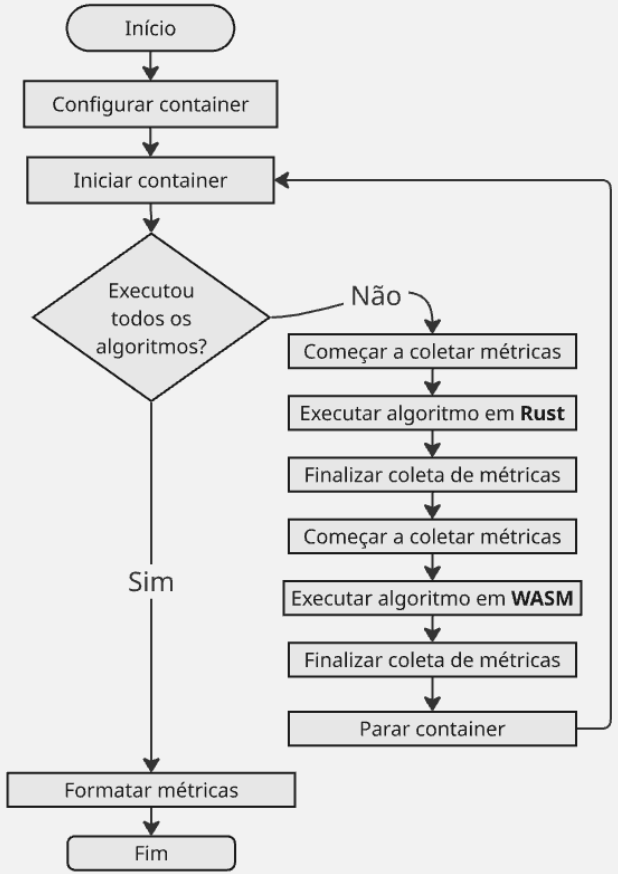
\includegraphics[scale=0.4]{media/diagrama-execucao-testes}
    \fonte{Os autores}
\end{figure}

\section{Ambiente de teste}

Com o objetivo de isolar o ambiente de execução, foram utilizados contêineres por meio do Docker, com quantidades controladas de CPUs e memória RAM, visando aumentar a reprodutibilidade dos experimentos.

Os testes foram realizados em 3 computadores diferentes, sendo posteriormente calculada a média dos resultados obtidos. Além disso, foram padronizadas as versões das tecnologias utilizadas em todos os computadores. A seguir, são apresentados os hardwares e os softwares utilizados.

\subsection{Hardwares}

Computador 1:

\begin{itemize}
    \item Sistema operacional: Ubuntu 24.04 (Noble);
    \item Kernel: Linux 6.17.0-35-generic;
    \item Processador: Intel i7 1165G7, 4 núcleos / 8 threads;
    \item Memória RAM: 16 GB LPDDR4 (8x2 GB) 4267 Mhz;
    \item Armazenamento: SSD NVMe de 1 TB Micron MTFDHBA1T0QFD.
\end{itemize}

Computador 2:

\begin{itemize}
    \item Sistema operacional: Ubuntu 24.04 LTS (Noble Numbat) via WSL 2;
    \item Kernel: Linux 6.6.87.2-microsoft-standard-WSL2;
    \item Processador: Intel Core i5-10300H, 4 núcleos / 8 threads;
    \item Memória RAM: 8 GB DDR (8x1 GB) 3200 Mhz;
    \item Armazenamento: SSD SATA de 500 GB KINGSTON SA400S37.
\end{itemize}

Computador 3:

\begin{itemize}
    \item Sistema operacional: Ubuntu 22.04 (Jammy) via WSL;
    \item Kernel: Linux 6.6.114.1-microsoft-standard-WSL2;
    \item Processador: AMD Ryzen 5 5600x, 6 núcleos / 12 threads;
    \item Memória RAM: 32 GB DDR4 (2x16 GB) 3200 Mhz;
    \item Armazenamento: SSD NVMe de 500 GB KINGSTON SNVS500G.
\end{itemize}

\subsection{Softwares}

\begin{itemize}
    \item Docker: versão 29.5.3;
    \item Docker Compose: versão v5.1.4;
    \item Rust: versão 1.95.0;
    \item wasm-pack: 0.14.0;
    \item wasm-bindgen: 0.2.121;
	\item Rayon: 1.8;
	\item Puppeteer: 24.43.1;
	\item Node.js: v24;
	\item npm: 10.9.4.
\end{itemize}

\section{Benchmarking}

Inicialmente, foi considerada a utilização de bibliotecas como Criterion e Hyperfine para a realização do \emph{benchmarking}. Entretanto, para simplificar a implementação, foram desenvolvidos \emph{scripts} responsáveis por automatizar a coleta de métricas dentro do contêiner Docker, além de código em Python para formatação e processamento dos dados coletados.

Essa abordagem também permitiu alterar parâmetros dos testes por meio de arquivos de configuração e realizar ajustes finos, buscando reduzir ao máximo interferências externas nos resultados.

\subsection{Avaliação}

Durante a avaliação, foram coletadas as métricas de tempo de execução, uso de memória ao longo do tempo e uso de CPU ao longo do tempo. Os \emph{scripts} desenvolvidos para a automação dos testes, a coleta dessas métricas e o código-fonte dos algoritmos utilizados estão disponíveis publicamente em um repositório no GitHub\footnote{Disponível em: \url{https://github.com/cmr-tcc/rust-wasm}.}.

Foi utilizado um intervalo de 25 milissegundos entre as coletas de memória e CPU. Como essas métricas representam o consumo de recursos do contêiner, foram considerados fatores como o uso de recursos em estado de espera (\emph{standby}) pelo contêiner e, no caso do Wasm, pelo Puppeteer, além da sobrecarga de carregamento da página \emph{web}. Para reduzir essa interferência, foi adotado um tempo de 10 segundos em estado ocioso (\emph{idle}) antes e depois de cada execução. Além disso, o contêiner era parado e então iniciado antes de cada execução para remover recursos residuais.

Para a análise de desempenho temporal, o \emph{overhead} percentual do WebAssembly em relação ao Rust nativo foi calculado pela Equação~\eqref{eq:overhead}:

\begin{equation}
\label{eq:overhead}
\text{\emph{overhead}}\,(\%) = \left( \frac{t_{\text{wasm}}}{t_{\text{rust}}} - 1 \right) \times 100
\end{equation}

\noindent em que $t_{\text{rust}}$ e $t_{\text{wasm}}$ representam os tempos médios de execução, em milissegundos, de cada ambiente.

Para a análise de memória, foram derivadas três métricas a partir das amostras coletadas, sendo $m_i$ o consumo de memória e $\mathit{cpu}_i$ a utilização de CPU na $i$-ésima amostra. O consumo de \emph{baseline} (Equação~\eqref{eq:baseline}) corresponde ao mínimo entre as amostras em que a utilização de CPU era inferior a 10\%, representando o consumo do contêiner em repouso. O consumo de pico (Equação~\eqref{eq:pico}) corresponde ao máximo entre as amostras com CPU acima de 80\%, representando o consumo durante a execução ativa. O consumo líquido é dado pela diferença entre pico e \emph{baseline} (Equação~\eqref{eq:liquido}):

\begin{equation}
\label{eq:baseline}
\text{\emph{baseline}} = \min \{\, m_i \mid \mathit{cpu}_i < 10\% \,\}
\end{equation}

\begin{equation}
\label{eq:pico}
\text{pico} = \max \{\, m_i \mid \mathit{cpu}_i > 80\% \,\}
\end{equation}

\begin{equation}
\label{eq:liquido}
\text{líquido} = \text{pico} - \text{\emph{baseline}}
\end{equation}

Essa distinção é necessária porque o contêiner Wasm mantém o Chrome Headless e o Puppeteer em execução permanente, elevando o \emph{baseline} a aproximadamente 200 MiB independentemente do algoritmo executado.
	\chapter{Análise dos resultados}
\label{cap:resultados}

As métricas coletadas foram analisadas com base no levantamento teórico realizado, buscando avaliar os aspectos de desempenho de maneira objetiva e fundamentada em cada cenário analisado. Os valores apresentados neste capítulo correspondem à média dos resultados obtidos nos três computadores descritos na metodologia.

Para o tempo de execução, foi comparado o resultado entre os dois ambientes, expressando a diferença como \emph{overhead} percentual e fator multiplicativo.

Para o consumo de memória, foram aplicadas as métricas de \emph{baseline}, pico e consumo líquido descritas anteriormente, a fim de isolar o consumo efetivo do algoritmo do \emph{overhead} fixo do ambiente de execução Wasm.

A utilização de CPU, embora coletada, não é apresentada como resultado, pois foi empregada apenas para identificar os períodos de execução, pelos motivos descritos na Seção~\ref{sec:consumo-memoria}.

\section{Tempo de Execução}

A Tabela~\ref{tab:tempo} apresenta os tempos médios de execução obtidos nos ambientes Rust e WebAssembly para os cinco algoritmos avaliados, além do \emph{overhead} percentual e do fator multiplicativo, calculados pelas Equações~\eqref{eq:overhead} e~\eqref{eq:fator} a partir das médias dos três computadores (Equação~\eqref{eq:media-computadores}). Os resultados mostram que o \emph{overhead} variou de 10,9\% a 126,9\%, indicando diferenças distintas entre os algoritmos avaliados. Em todos os casos, o WebAssembly apresentou tempo de execução maior que o Rust nativo.
\begin{table}[H]
    \caption{ Comparativo de tempo de execução médio (ms) }
    \label{tab:tempo}
    \centering
    \setlength{\tabcolsep}{5pt}
    \begin{tabular}{ccccccc}
        \hline
        Algoritmo &Rust (ms) &Wasm (ms) &Overhead (\%) &Fator \\
        \hline
        fannkuch-redux &21.226,7 &23.539,7 &10,9 &1,109x \\
        \hline
        spectral-norm &1.271,7 &1.436,2 &12,9 &1,129x \\
        \hline
        fasta &1.701,5 &2.061,5 &21,2 &1,212x \\
        \hline
        n-body &1.907,7 &3.227,3 &69,2 &1,692x \\
        \hline
        mandelbrot &3.253,5 &7.381,7 &126,9 &2,269x \\
        \hline
    \end{tabular}
    \fonte{Os autores}
\end{table}

Os menores \emph{overheads} foram observados em fannkuch-redux e spectral-norm, com 10,9\% e 12,9\%, respectivamente. Em contraste, n-body e mandelbrot apresentaram as maiores diferenças, com 69,2\% e 126,9\%. A Figura~\ref{fig:grafico-tempo-benchmarking} permite visualizar essas diferenças entre os tempos médios de execução nos dois ambientes.

\begin{figure}[!htb]
	\centering
	\caption{Comparativo de tempo de execução médio}
    \label{fig:grafico-tempo-benchmarking}
	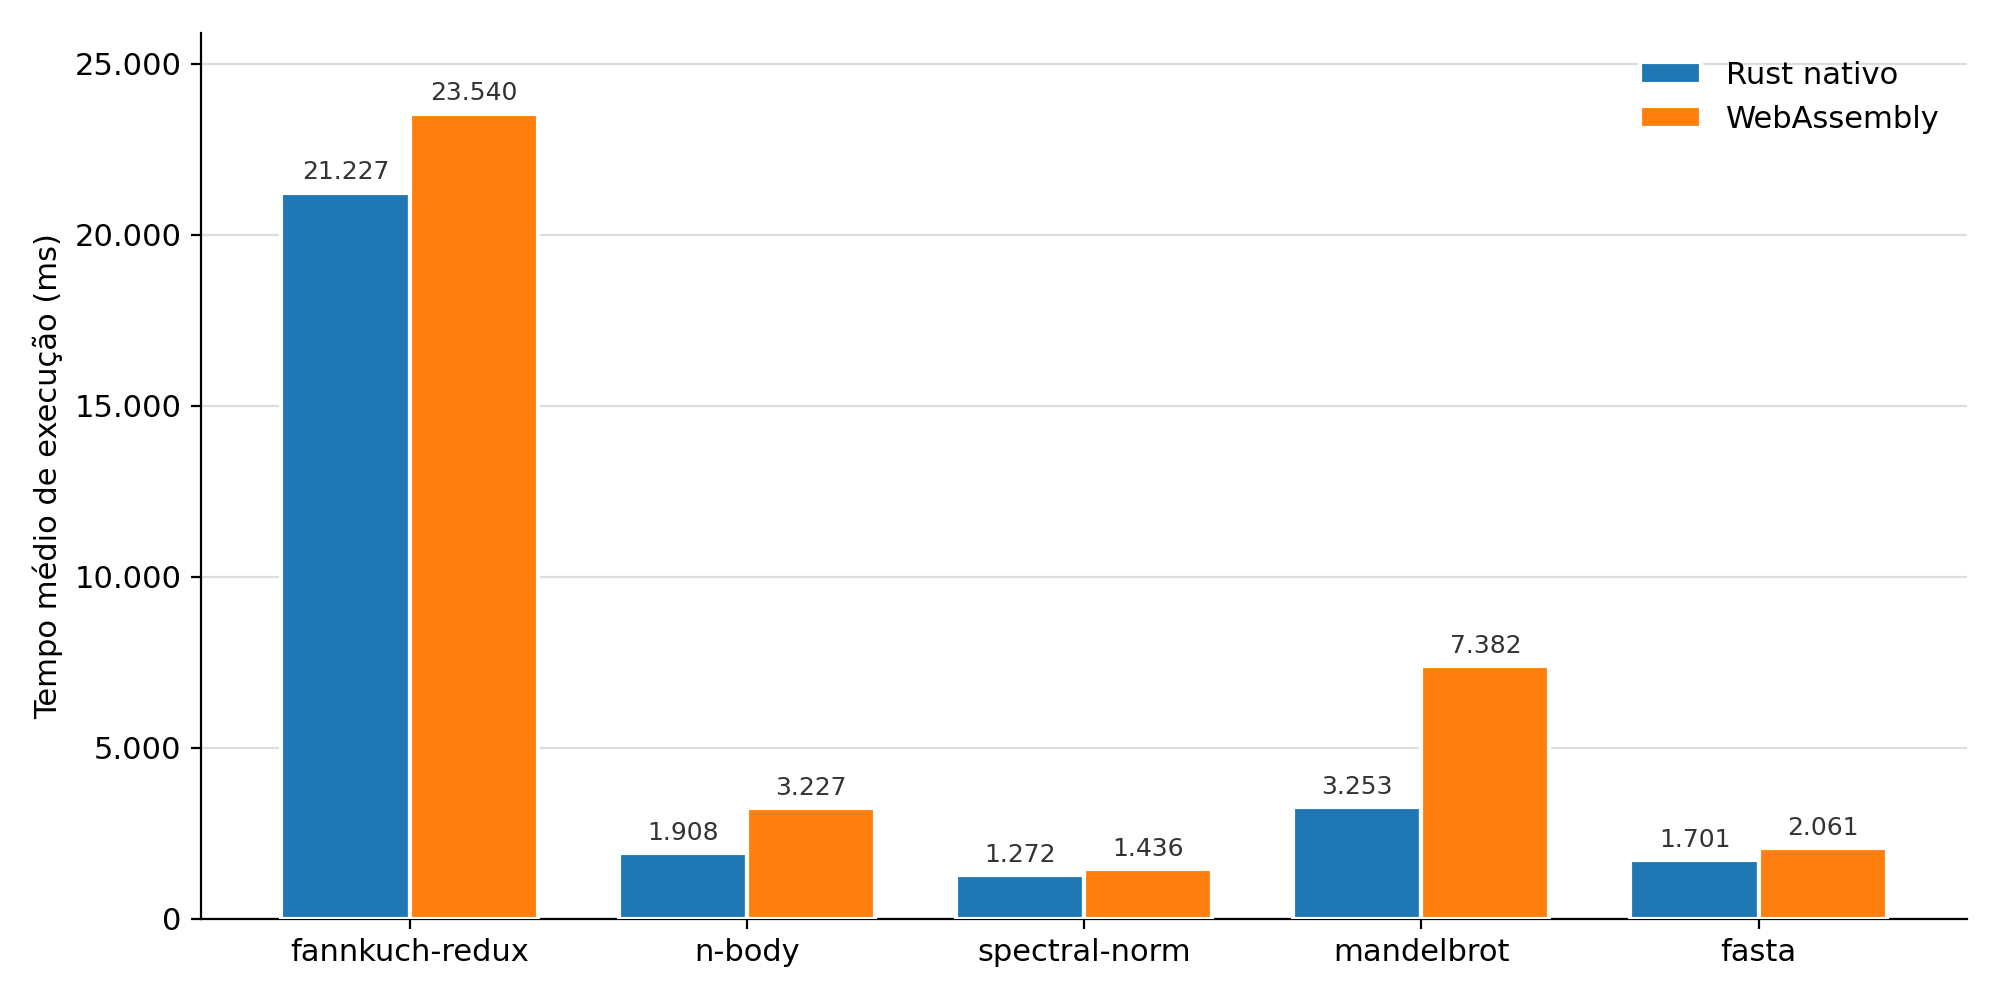
\includegraphics[width=\textwidth]{media/grafico-tempo-benchmarking}
    \fonte{Os autores}
\end{figure}

O algoritmo fannkuch-redux registrou o menor \emph{overhead}, correspondente a 10,9\%, ou fator 1,109x. Trata-se de um algoritmo baseado em permutações de vetores de inteiros de tamanho fixo, com operações predominantemente inteiras.

O spectral-norm apresentou \emph{overhead} de 12,9\%. O algoritmo realiza operações de ponto flutuante de dupla precisão em laços sobre vetores.

O algoritmo fasta obteve \emph{overhead} de 21,2\%. Sua execução envolve a geração de números pseudoaleatórios, consultas a tabelas de probabilidade acumulada e a escrita das sequências geradas em blocos de memória.

O n-body registrou \emph{overhead} de 69,2\%. A simulação envolve cálculos iterativos de forças gravitacionais entre cinco corpos, com uso intensivo de operações de ponto flutuante de dupla precisão, incluindo raízes quadradas, sobre um conjunto reduzido de dados.

O mandelbrot apresentou o maior \emph{overhead} observado, correspondente a 126,9\%. Nesse cenário, o tempo de execução em WebAssembly foi mais que o dobro do observado na execução nativa. O algoritmo realiza processamento intensivo de ponto flutuante de dupla precisão e grava o resultado em um \emph{buffer} de \emph{bits}.

Considerando todos os algoritmos avaliados, o \emph{overhead} médio foi de 48,2\% (Equação~\eqref{eq:media-overhead}), enquanto a mediana foi de 21,2\% (Equação~\eqref{eq:mediana-overhead}). A diferença entre essas métricas indica que os casos extremos, especialmente o mandelbrot, exercem influência significativa sobre a média geral dos resultados.

Os valores absolutos de tempo variaram entre os três computadores, que possuem configurações de \emph{hardware} e sistema operacional distintas, e o \emph{overhead} de alguns algoritmos também oscilou entre as máquinas, como no fannkuch-redux, entre 4,0\% e 18,0\%, e no spectral-norm, entre 7,6\% e 26,6\%. Ainda assim, a separação entre os grupos se manteve em todas elas: mandelbrot e n-body registraram os maiores \emph{overheads} nos três computadores, enquanto fannkuch-redux, spectral-norm e fasta permaneceram abaixo de 27\%.

\section{Uso de Memória}

As métricas de \emph{baseline}, pico e consumo líquido foram calculadas pelas Equações~\eqref{eq:baseline} a~\eqref{eq:liquido} para cada computador e consolidadas pela média entre eles (Equação~\eqref{eq:media-computadores}). As Tabelas~\ref{tab:memoria-rust} e~\ref{tab:memoria-wasm} apresentam os resultados obtidos.

\begin{table}[!h]
    \caption{Consumo de memória do executável Rust (MiB)}
    \label{tab:memoria-rust}
    \centering
    \setlength{\tabcolsep}{6pt}
    \begin{tabular}{lccc}
        \hline
        Algoritmo & Base & Pico & Líquido \\
        \hline
        fannkuch-redux  & 16,6 & 17,7 & 1,1 \\
        n-body          & 7,9  & 8,6  & 0,7 \\
        spectral-norm   & 8,1  & 9,0  & 1,0 \\
        mandelbrot      & 8,0  & 40,4 & 32,3 \\
        fasta           & 7,9  & 9,1  & 1,2 \\
        \hline
    \end{tabular}
    \fonte{Os autores}
\end{table}

\begin{table}[!h]
    \caption{Consumo de memória do executável WebAssembly (MiB)}
    \label{tab:memoria-wasm}
    \centering
    \setlength{\tabcolsep}{6pt}
    \begin{tabular}{lccc}
        \hline
        Algoritmo & Base & Pico & Líquido \\
        \hline
        fannkuch-redux  & 218,6 & 237,0 & 18,4 \\
        n-body          & 209,9 & 213,7 & 3,8 \\
        spectral-norm   & 209,6 & 211,7 & 2,2 \\
        mandelbrot      & 209,9 & 245,9 & 36,1 \\
        fasta           & 209,9 & 212,7 & 2,8 \\
        \hline
    \end{tabular}
    \fonte{Os autores}
\end{table}

O \emph{baseline} do ambiente Rust situou-se entre 7,9 MiB e 16,6 MiB, refletindo principalmente o consumo do contêiner em estado ocioso. O valor mais alto, observado no fannkuch-redux, decorre de um dos computadores, que registrou 32,1 MiB nessa execução, enquanto os demais ficaram próximos de 9 MiB. No ambiente WebAssembly, os valores de \emph{baseline} variaram entre 209,6 MiB e 218,6 MiB, em razão da execução permanente do Chrome Headless e do Puppeteer.

Dessa forma, a comparação direta entre os valores totais de memória não é adequada para avaliar exclusivamente o impacto dos algoritmos. Por esse motivo, a análise foi concentrada no consumo líquido de memória.

Considerando essa métrica, o Rust apresentou consumo líquido entre 0,7 MiB e 1,2 MiB em quatro dos cinco algoritmos: fannkuch-redux, n-body, spectral-norm e fasta. A exceção foi o mandelbrot, com 32,3 MiB, valor praticamente idêntico nos três computadores e compatível com o \emph{buffer} de saída alocado pelo algoritmo, que armazena um \emph{bit} por \emph{pixel} de uma imagem de 16.000 por 16.000 \emph{pixels}, totalizando cerca de 30,5 MiB.

No WebAssembly, o consumo líquido ficou entre 2,2 MiB e 3,8 MiB para n-body, spectral-norm e fasta, ligeiramente acima dos valores do Rust nativo. O mandelbrot também apresentou o maior consumo nesse ambiente, com 36,1 MiB, valor igualmente compatível com o \emph{buffer} de saída, que no WebAssembly é alocado na memória linear do módulo. O fannkuch-redux registrou 18,4 MiB, porém com grande variação entre os computadores, de 4,2 MiB a 39,5 MiB.

De modo geral, o consumo líquido do WebAssembly foi maior que o do Rust nativo em todos os algoritmos.

\section{Síntese comparativa}

Os resultados mostram que o Rust nativo foi mais rápido em todos os algoritmos e que o \emph{overhead} do WebAssembly variou de forma expressiva conforme o algoritmo. Fannkuch-redux, spectral-norm e fasta ficaram entre 10,9\% e 21,2\%, enquanto n-body e mandelbrot chegaram a 69,2\% e 126,9\%, separação que se manteve nos três computadores.

Também o ambiente WebAssembly exige, em repouso, cerca de 200 MiB a mais que o ambiente nativo, com \emph{baseline} de cerca de 210 MiB, contra 7,9 MiB a 16,6 MiB no Rust, para manter o Chrome Headless através do Puppeteer em execução, valor praticamente constante entre os algoritmos e independente da carga processada, tornando a comparação direta com o ambiente nativo inadequada. Por esse motivo, a análise de consumo de memória foi concentrada no consumo líquido, que isolou o impacto do algoritmo em execução. Por essa métrica, os dois ambientes apresentaram consumo reduzido na maioria dos algoritmos, com o WebAssembly ligeiramente acima do Rust nativo, e o maior consumo em ambos foi o do mandelbrot, determinado pelo tamanho do \emph{buffer} de saída.

\section{Limitações do estudo}

Há limitações que devem ser consideradas neste estudo:

\begin{itemize}
    \item Nos testes realizados, a variável de ambiente \texttt{RAYON\_NUM\_THREADS} foi fixada em 1, restringindo a execução de algoritmos que utilizam a biblioteca \emph{Rayon} a uma única \emph{thread}, mesmo naqueles casos em que o processamento paralelo poderia representar ganhos de desempenho. Essa restrição foi necessária em razão de erros encontrados na compilação da biblioteca \emph{wasm-bindgen-rayon} para o ambiente WebAssembly, e foi replicada no ambiente Rust nativo para manter a padronização entre as comparações.
    \item Estudos futuros poderiam empregar ambientes de execução WebAssembly independentes de navegador, como \emph{Wasmer} e \emph{Wasmtime}, permitindo isolar de forma mais precisa o desempenho do código WebAssembly.
    \item A avaliação do ambiente WebAssembly limitou-se ao navegador Google Chrome, controlado por meio do Puppeteer, o que restringe a generalização dos resultados obtidos. Diferentes navegadores utilizam motores de execução WebAssembly distintos, cada um com estratégias próprias de otimização, o que pode alterar significativamente os resultados de desempenho.
\end{itemize}

	\chapter{CONSIDERAÇÕES FINAIS}

Este trabalho realizou uma análise comparativa entre a execução nativa de código Rust e sua execução compilada para WebAssembly, avaliando os impactos em tempo de execução e consumo de memória. A utilização de CPU também foi coletada, mas mostrou-se pouco informativa para a comparação, pelos motivos descritos na Seção~\ref{sec:consumo-memoria}, sendo utilizada apenas para identificar os períodos de execução.

Para embasar essa análise, foram abordados os fundamentos da linguagem Rust e as características do WebAssembly na revisão da literatura. Além disso, na etapa prática foram selecionados, do The Computer Language Benchmarks Game, 5 algoritmos de diferentes classes de problemas, implementados em Rust, portados para WebAssembly e executados em ambiente controlado via Docker em 3 máquinas distintas. Os resultados mostraram que o Rust nativo foi mais rápido que o WebAssembly em todos os algoritmos avaliados, com \emph{overhead} do WebAssembly entre 10,9\%, no fannkuch-redux, e 126,9\%, no mandelbrot, e mediana de 21,2\%. A análise de memória evidenciou que parte do consumo do ambiente WebAssembly não está associada à execução dos algoritmos, mas ao ambiente de execução, que mantém componentes como o Chrome Headless e o Puppeteer em funcionamento contínuo e eleva o consumo de memória em repouso para cerca de 210 MiB.

Diante disso, a utilização das métricas de \emph{baseline} e consumo líquido mostrou-se fundamental para isolar o impacto real dos algoritmos, permitindo uma análise mais precisa e justa entre os ambientes. Por essa métrica, o consumo líquido dos dois ambientes foi reduzido na maioria dos algoritmos, com o WebAssembly ligeiramente acima do Rust nativo, e o maior consumo em ambos foi o do mandelbrot, determinado pelo tamanho do \emph{buffer} de saída. Observou-se ainda que o \emph{overhead} de tempo varia conforme o padrão de acesso à memória, indicando que algoritmos com acesso sequencial e previsível tendem a apresentar desempenho mais próximo do nativo, enquanto aqueles com acesso irregular ou escrita intensiva apresentam maior degradação de desempenho.

Conclui-se, portanto, que o WebAssembly representa uma alternativa viável à execução nativa para aplicações Rust executadas no navegador com acesso predominantemente sequencial à memória, cenário em que o custo adicional ficou entre 10,9\% e 21,2\%. Para cargas com escrita intensiva ou acesso irregular à memória, o custo pode superar o dobro do tempo nativo, e a execução nativa segue mais indicada quando o desempenho é o principal requisito.

Como limitação, os algoritmos foram executados com uma única \emph{thread} nos dois ambientes, pois não foi possível habilitar o processamento paralelo no WebAssembly. Como trabalhos futuros, sugere-se avaliar a execução multi-\emph{thread} no navegador, ampliar o conjunto de algoritmos e comparar outros mecanismos de execução de WebAssembly.

	
	\postextual
	% espaçamento entre o título e o primeiro parágrafo do texto
	\setlength\afterchapskip{18pt}
	\bibliographystyle{referencias-style}
	\bibliography{referencias}

% apêndices
% \begin{apendicesenv}
	
% 	\renewcommand{\thetable}{\Alph{chapter}\arabic{table}}
% 	\setcounter{table}{0}
% 	\clearpage
% 		\begingroup
% 		\makeatletter
% 		\let\clearpage\relax
% 		\vspace*{\fill}
% 		\vspace*{\dimexpr-50\p@-\baselineskip}
% 		\chapter{Análise Estatística}
% 		\vspace*{\fill}
% 		\endgroup 
% 	\clearpage
	
% 	\lipsum[50]
	
% \end{apendicesenv}

% anexos
% \begin{anexosenv}

% 	\chapter{Laudo técnico}

% 	\lipsum[30]
		
% \end{anexosenv}

% índice remissivo
\phantompart
\printindex

\end{document}